\chapter{Software Requirement Specification}

\section{Product Overview}

The \textbf{Personalized Career Orientation \& Learning Roadmap Platform for Software Engineering Students} is an intelligent web-based software platform designed to support Software Engineering students in planning their academic development and preparing for future careers. The system replaces the traditional approach of manually searching for career information, collecting learning resources from multiple websites, and creating self-designed learning plans without structured guidance. Instead, it provides a centralized platform that integrates AI-powered career consultation, personalized learning roadmap generation, skill gap analysis, portfolio management, and technology trend analysis into a single environment. The platform enables students to identify suitable career paths, monitor learning progress, build professional portfolios, and receive personalized recommendations based on their academic background, technical skills, and career aspirations.  

The context diagram below illustrates the external entities and system interfaces for \textbf{Release 1.0} of the proposed platform. In this release, the system interacts with students, academic counselors, industry mentors, administrators, Artificial Intelligence services, GitHub, Google Authentication, and external job market data providers to deliver personalized career orientation and learning support. Future releases are expected to incorporate additional features such as internship recommendation, online certification integration, collaboration among students, mobile applications, and deeper integration with university information systems to provide a more comprehensive learning and career development ecosystem. 

\begin{figure}[H]
    \centering
    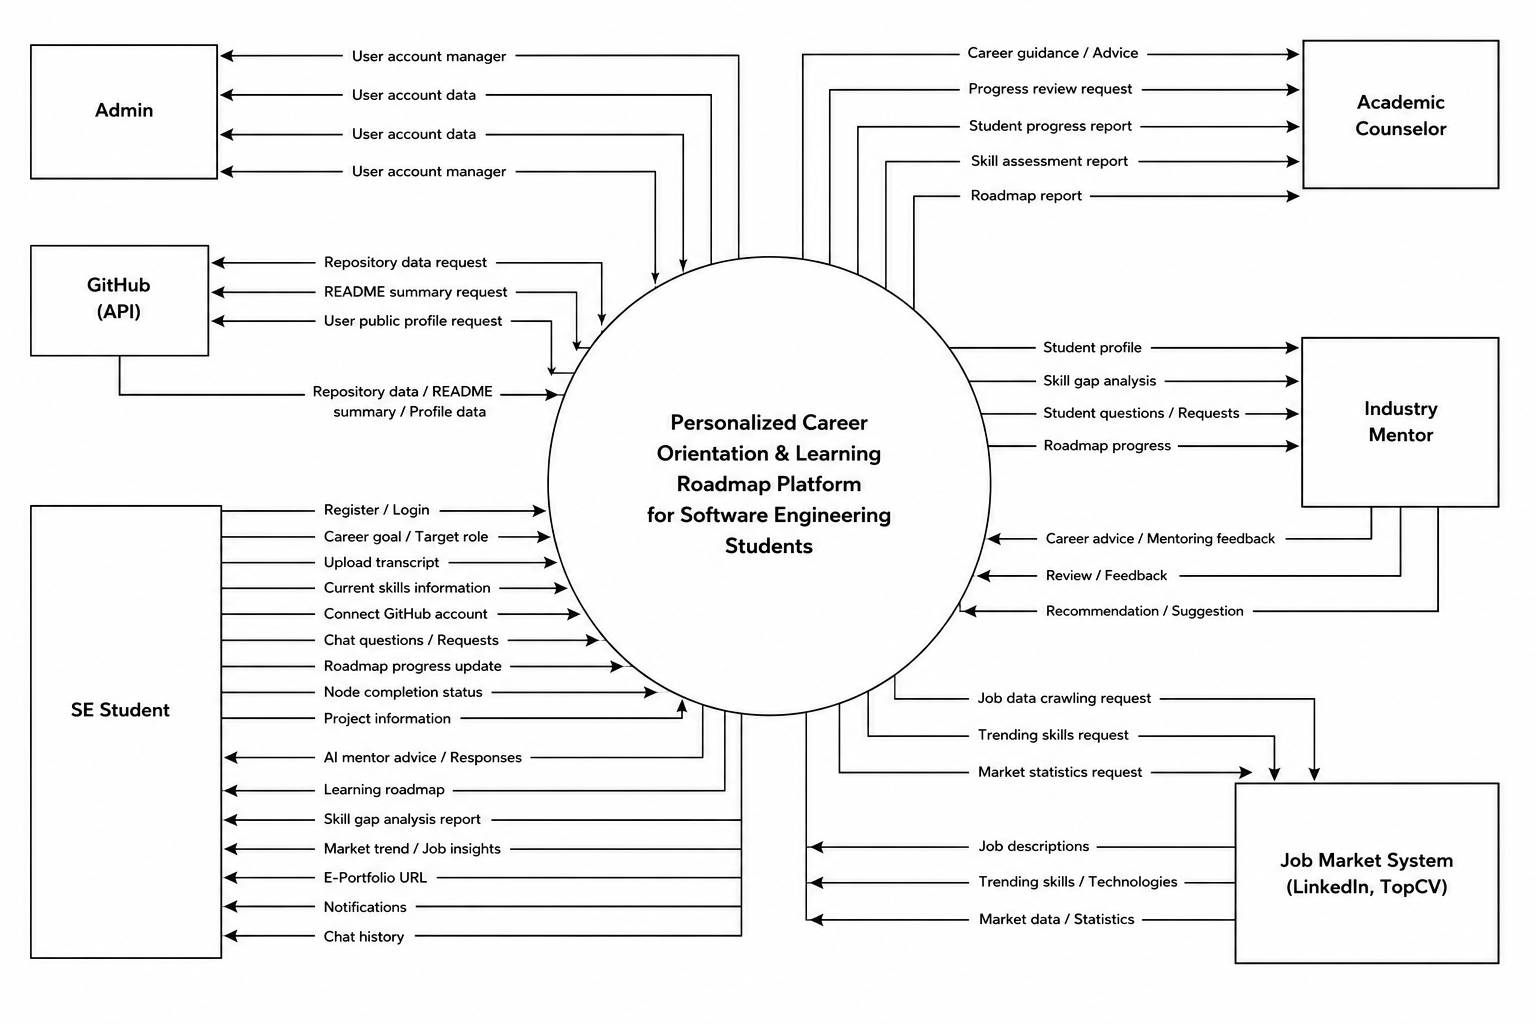
\includegraphics[width=\textwidth]{images/context_diagram.png}
    \caption{Context Diagram}
    \label{fig:context_diagram}
\end{figure}

\section{User Requirements}

This section describes the users who interact with the system and the major use cases supported by the Personalized Career Orientation and Learning Roadmap Platform. These requirements define what each actor expects from the system and serve as the foundation for the functional requirements presented in the next section.

\subsection{Actors}

\renewcommand{\arraystretch}{1.5}

\begin{longtable}{|>{\centering\arraybackslash}p{0.8cm}|>{\centering\arraybackslash}p{3.5cm}|p{10cm}|}
\hline
\rowcolor[HTML]{F4D7D7}
\textbf{\#} & \textbf{Actor} & \textbf{Description} \\
\hline
\endfirsthead
\hline
\endhead

1 &
\textbf{Administrator}
&
Responsible for managing the entire platform, including user account management, role assignment, authentication settings, AI service configuration, learning resource management, and monitoring system performance. The Administrator ensures platform security, maintains data integrity, and guarantees reliable system operation.
\\
\hline

2 &
\textbf{SE Student}
&
The primary user of the platform. Students create and manage personal profiles, define target career roles, upload academic transcripts, connect GitHub accounts, perform skill assessments, interact with the AI Virtual Mentor, follow personalized learning roadmaps, monitor skill gap analysis, explore job market trends, and manage AI-generated e-portfolios.
\\
\hline

3 &
\textbf{Academic Counselor}
&
Supports students throughout their academic and career development. Academic Counselors review students' learning progress, evaluate roadmap completion, analyze skill development, recommend suitable learning resources, provide career guidance, and assist students in selecting appropriate Software Engineering career paths.
\\
\hline

4 &
\textbf{Industry Mentor}
&
Represents experienced professionals from the software industry who provide practical career guidance and technical mentoring. Industry Mentors review student profiles, evaluate skill gap reports, answer career-related questions, recommend industry best practices, suggest learning priorities, and provide feedback based on current recruitment demands and real-world software development experience.
\\
\hline

\end{longtable}

\subsection{Use Cases}

\subsubsection{Diagram(s)}

\begin{figure}[H]
    \centering
    
\includegraphics[width=\textwidth]{images/usecase_diagram.png}
    \caption{Use Case Diagram of the Personalized Career Orientation and Learning Roadmap Platform}
    \label{fig:usecase}
\end{figure}

\subsubsection{Descriptions}

The following use cases describe the authentication and account management
functions that are shared by all users of the platform. These functions
ensure secure access, account protection, and identity verification before
users interact with the Personalized Career Orientation and Learning Roadmap
Platform.

\renewcommand{\arraystretch}{1.4}

\begin{longtable}{|>{\centering\arraybackslash}p{1cm}|p{4cm}|p{3.3cm}|p{7.2cm}|}
\hline
\rowcolor[HTML]{F4D7D7}
\textbf{ID} &
\textbf{Use Case} &
\textbf{Actors} &
\textbf{Use Case Description}
\\
\hline
\endfirsthead

\hline
\endhead

UC01 &
Register &
SE Student &
Create a new account.
\\
\hline

UC02 &
Login &
All authenticated users &
Login to the platform.
\\
\hline

UC03 &
Login with Google &
SE Student &
Authenticate using Google OAuth.
\\
\hline

UC04 &
Logout &
All authenticated users &
Logout from the system.
\\
\hline

UC05 &
Reset Password &
All users &
Recover forgotten password.
\\
\hline

UC06 &
Change Password &
Authenticated users &
Change current password.
\\
\hline

UC07 &
View Profile &
Student &
View personal profile.
\\
\hline

UC08 &
Update Profile &
Student &
Edit personal information.
\\
\hline

UC09 &
Upload Avatar &
Student &
Upload profile picture.
\\
\hline

UC10 &
Upload Transcript &
Student &
Upload academic transcript.
\\
\hline

UC11 &
View Transcript &
Student &
View uploaded transcript.
\\
\hline

UC12 &
Update Transcript &
Student &
Replace transcript.
\\
\hline

UC13 &
Delete Transcript &
Student &
Remove transcript.
\\
\hline

UC14 &
Select Career Goal &
Student &
Select desired career role.
\\
\hline

UC15 &
View Career Roles &
Student &
Browse available career paths.
\\
\hline

UC16 &
Connect GitHub &
Student &
Link GitHub account.
\\
\hline

UC17 &
Disconnect GitHub &
Student &
Remove GitHub account.
\\
\hline

UC18 &
View GitHub Projects &
Student &
Display repositories.
\\
\hline

UC19 &
Chat with AI Mentor &
Student &
Ask AI questions.
\\
\hline

UC20 &
Receive AI Advice &
Student &
Receive AI responses.
\\
\hline

UC21 &
View Personalized Roadmap &
Student &
Display roadmap.
\\
\hline

UC22 &
Update Roadmap Progress &
Student &
Update completed skills.
\\
\hline

UC23 &
View Skill Gap Report &
Student &
Review missing skills.
\\
\hline

UC24 &
View Learning Progress &
Student &
Monitor completion percentage.
\\
\hline

UC25 &
Search Learning Resources &
Student &
Search learning materials.
\\
\hline

UC26 &
View Recommended Courses &
Student &
Display suggested courses.
\\
\hline

UC27 &
View Market Trends &
Student &
View technology trends.
\\
\hline

UC28 &
View Job Insights &
Student &
Browse recruitment demand.
\\
\hline

UC29 &
Generate Portfolio &
Student &
Generate e-portfolio.
\\
\hline

UC30 &
View Portfolio &
Student &
Display portfolio.
\\
\hline

UC31 &
Share Portfolio &
Student &
Share public portfolio.
\\
\hline

UC32 &
Download Portfolio &
Student &
Export PDF portfolio.
\\
\hline

UC33 &
View Notifications &
Student &
Receive notifications.
\\
\hline

UC34 &
View Student Profile &
Counselor &
View student information.
\\
\hline

UC35 &
Review Transcript &
Counselor &
Review transcript.
\\
\hline

UC36 &
Review Skill Gap &
Counselor &
Analyze skill gaps.
\\
\hline

UC37 &
Review Learning Progress &
Counselor &
Monitor progress.
\\
\hline

UC38 &
Recommend Career Path &
Counselor &
Suggest career path.
\\
\hline

UC39 &
Recommend Learning Plan &
Counselor &
Recommend roadmap improvements.
\\
\hline

UC40 &
Comment Learning Plan &
Counselor &
Leave comments.
\\
\hline

UC41 &
Send Feedback &
Counselor &
Send feedback.
\\
\hline

UC42 &
View Reports &
Counselor &
View progress reports.
\\
\hline

UC43 &
Manage Consultation &
Counselor &
Schedule consultation.
\\
\hline

UC44 &
View Student Portfolio &
Mentor &
View portfolio.
\\
\hline

UC45 &
Review GitHub Repository &
Mentor &
Review repositories.
\\
\hline

UC46 &
Review Projects &
Mentor &
Evaluate projects.
\\
\hline

UC47 &
Recommend Technologies &
Mentor &
Suggest technologies.
\\
\hline

UC48 &
Provide Technical Advice &
Mentor &
Give technical guidance.
\\
\hline

UC49 &
Evaluate Progress &
Mentor &
Evaluate learning progress.
\\
\hline

UC50 &
Comment Portfolio &
Mentor &
Comment portfolio.
\\
\hline

UC51 &
View Skill Gap Report &
Mentor &
Review skill analysis.
\\
\hline

UC52 &
Recommend Industry Skills &
Mentor &
Recommend market skills.
\\
\hline

UC53 &
Send Mentoring Feedback &
Mentor &
Submit mentoring feedback.
\\
\hline

UC54 &
Manage Users &
Administrator &
Manage user accounts.
\\
\hline

UC55 &
Add User &
Administrator &
Create user.
\\
\hline

UC56 &
Update User &
Administrator &
Update user.
\\
\hline

UC57 &
Delete User &
Administrator &
Delete user.
\\
\hline

UC58 &
View Users &
Administrator &
View users.
\\
\hline

UC59 &
Manage Career Roles &
Administrator &
CRUD career roles.
\\
\hline

UC60 &
Manage Skill Nodes &
Administrator &
CRUD skill tree.
\\
\hline

UC61 &
Manage Skill Categories &
Administrator &
Manage skill groups.
\\
\hline

UC62 &
Manage Learning Resources &
Administrator &
CRUD resources.
\\
\hline

UC63 &
Manage Courses &
Administrator &
CRUD courses.
\\
\hline

UC64 &
Manage Job Trend Data &
Administrator &
Update market data.
\\
\hline

UC65 &
Manage AI Models &
Administrator &
Configure AI.
\\
\hline

UC66 &
Configure Recommendation Engine &
Administrator &
Tune recommendation engine.
\\
\hline

UC67 &
Manage Notifications &
Administrator &
Send notifications.
\\
\hline

UC68 &
View Analytics &
Administrator &
View dashboards.
\\
\hline

UC69 &
Generate Reports &
Administrator &
Export reports.
\\
\hline

UC70 &
Backup Database &
Administrator &
Backup system.
\\
\hline

UC71 &
Restore Database &
Administrator &
Restore data.
\\
\hline

UC72 &
Analyze Transcript &
AI Engine &
Analyze transcript.
\\
\hline

UC73 &
Analyze GitHub Repository &
AI Engine &
Analyze GitHub.
\\
\hline

UC74 &
Analyze Skill Gap &
AI Engine &
Detect missing skills.
\\
\hline

UC75 &
Generate Personalized Roadmap &
AI Engine &
Generate roadmap.
\\
\hline

UC76 &
Recommend Courses &
AI Engine &
Recommend learning resources.
\\
\hline

UC77 &
Generate Portfolio Summary &
AI Engine &
Summarize portfolio.
\\
\hline

UC78 &
Authenticate User &
Google OAuth &
Verify identity.
\\
\hline

UC79 &
Retrieve Repository &
GitHub API &
Retrieve repositories.
\\
\hline

UC80 &
Retrieve README &
GitHub API &
Retrieve README.
\\
\hline

UC81 &
Retrieve Tech Stack &
GitHub API &
Retrieve technologies.
\\
\hline

UC82 &
Retrieve Job Data &
Job Portal API &
Retrieve recruitment data.
\\
\hline

UC83 &
Analyze Market Trends &
Job Portal API &
Analyze job market.
\\
\hline

UC84 &
Retrieve Salary Statistics &
Job Portal API &
Retrieve salary data.
\\
\hline

\end{longtable}

\section{Functional Requirements}

\subsection{System Functional Requirements}

\subsubsection{Screens Flow}

\textbf{Administrator Screen Flow}

\begin{figure}[H]
    \centering
    
\includegraphics[width=\textwidth]{images/Administrator_ScreenFlow.png}
    \caption{Administrator Screen Flow}
    \label{fig:administrator_screenflow}
\end{figure}

\clearpage

\textbf{Student Screen Flow}

\begin{figure}[H]
    \centering
    
\includegraphics[width=\textwidth]{images/Student_ScreenFlow.png}
    \caption{Student Screen Flow}
    \label{fig:student_screenflow}
\end{figure}

\textbf{Academic Counselor Screen Flow}

\begin{figure}[H]
    \centering
    
\includegraphics[width=\textwidth]{images/AcademicCounselor_ScreenFlow.png}
    \caption{Academic Counselor Screen Flow}
    \label{fig:academiccounselor_screenflow}
\end{figure}

\clearpage

\textbf{Industry Mentor Screen Flow}

\begin{figure}[H]
    \centering
    
\includegraphics[width=\textwidth]{images/IndustryMentor_ScreenFlow.png}
    \caption{Industry Mentor Screen Flow}
    \label{fig:industrymentor_screenflow}
\end{figure}

\subsubsection{Screen Descriptions}

\renewcommand{\arraystretch}{1.4}

\begin{longtable}{|>{\centering\arraybackslash}p{0.8cm}|p{3.2cm}|p{3.5cm}|p{8cm}|}
\hline
\rowcolor[HTML]{F4D7D7}
\textbf{\#} &
\textbf{Feature} &
\textbf{Screen} &
\textbf{Description}
\\
\hline
\endfirsthead

\hline
\endhead

1 &
Authentication &
Login Page &
Allows Administrator, Academic Counselor, Industry Mentor and SE Student to authenticate using email/password or Google OAuth before accessing the system.
\\
\hline

2 &
Dashboard &
Administrator Dashboard &
Displays system statistics, user activities, AI recommendation status, learning resources and administrative shortcuts.
\\
\hline

3 &
User Management &
Manage Users &
Allows administrators to create, search, update, delete and manage user accounts together with role assignment.
\\
\hline

4 &
Create User &
Create User &
Allows administrators to register new student, counselor or mentor accounts.
\\
\hline

5 &
View Users &
View Users &
Displays all registered users with filtering and searching functions.
\\
\hline

6 &
Update User &
Update User &
Allows administrators to modify user profile information and account status.
\\
\hline

7 &
Delete User &
Delete User &
Allows administrators to remove inactive or unnecessary user accounts.
\\
\hline

8 &
Career Management &
Manage Career Roles &
Allows administrators to create, update and maintain Software Engineering career roles.
\\
\hline

9 &
Skill Management &
Manage Skill Nodes &
Allows administrators to organize the hierarchical Software Engineering skill tree.
\\
\hline

10 &
Course Management &
Manage Courses &
Allows administrators to manage recommended courses and learning resources.
\\
\hline

11 &
Learning Resources &
Manage Learning Resources &
Allows administrators to add, update and remove books, MOOCs, tutorials and documentation.
\\
\hline

12 &
Market Data &
Manage Job Trend Data &
Allows administrators to synchronize and maintain recruitment market information collected from Job Portal APIs.
\\
\hline

13 &
AI Configuration &
Configure AI Engine &
Allows administrators to configure AI recommendation parameters and external AI services.
\\
\hline

14 &
Analytics &
View Analytics &
Displays statistical reports, recommendation accuracy and platform usage.
\\
\hline

15 &
Reports &
Generate Reports &
Allows administrators to export system reports into PDF or Excel.
\\
\hline

16 &
Notifications &
Send Notifications &
Allows administrators to broadcast announcements and notifications to users.
\\
\hline

17 &
Database Backup &
Backup Database &
Creates backup copies of the system database for disaster recovery.
\\
\hline

18 &
Database Restore &
Restore Database &
Restores system data from previously created backups.
\\
\hline

19 &
Logout &
Logout &
Ends the administrator session securely.
\\
\hline

20 &
Profile Management &
Student Dashboard &
Displays the student's personalized dashboard including learning progress, career roadmap, AI recommendations, GitHub integration status and recent notifications.
\\
\hline

21 &
Profile &
View Profile &
Allows students to view their personal information, academic information and career preferences.
\\
\hline

22 &
Profile &
Update Profile &
Allows students to update personal information such as fullname, phone number, biography and career interests.
\\
\hline

23 &
Avatar Management &
Upload Avatar &
Allows students to upload or replace their profile picture.
\\
\hline

24 &
Career Planning &
Select Career Goal &
Allows students to choose their desired Software Engineering career path for AI recommendation.
\\
\hline

25 &
Career Planning &
View Career Roles &
Displays available Software Engineering career paths together with required skills and descriptions.
\\
\hline

26 &
GitHub Integration &
Connect GitHub &
Allows students to connect their GitHub account for automatic repository analysis.
\\
\hline

27 &
GitHub Integration &
View GitHub Projects &
Displays public repositories, programming languages and project information retrieved from GitHub.
\\
\hline

28 &
GitHub Integration &
Disconnect GitHub &
Allows students to remove GitHub account integration from the platform.
\\
\hline

29 &
AI Virtual Mentor &
Chat with AI &
Allows students to ask questions related to programming, learning plans and career orientation.
\\
\hline

30 &
AI Recommendation &
Receive AI Advice &
Displays personalized recommendations generated by the AI Recommendation Engine.
\\
\hline

31 &
Learning Roadmap &
View Roadmap &
Displays the personalized learning roadmap generated based on career goals and current skills.
\\
\hline

32 &
Learning Roadmap &
Update Progress &
Allows students to mark completed skills, courses and certifications.
\\
\hline

33 &
Skill Analysis &
Skill Gap Report &
Displays missing skills required for the selected Software Engineering career path.
\\
\hline

34 &
Learning Resources &
Learning Resources &
Displays recommended books, online courses, documentation and tutorials suggested by the AI engine.
\\
\hline

35 &
Portfolio &
Generate Portfolio &
Automatically generates an AI-powered e-Portfolio based on academic records, GitHub projects and completed skills.
\\
\hline

36 &
Portfolio &
View Portfolio &
Allows students to preview, download and share their professional e-Portfolio.
\\
\hline

37 &
Job Market Analysis &
Market Trends &
Displays current Software Engineering technology trends and hiring demands collected from Job Portal APIs.
\\
\hline

38 &
Job Market Analysis &
Job Insights &
Displays recruitment statistics, required technologies, salary trends and industry demand.
\\
\hline

39 &
Notifications &
Notifications &
Displays system notifications, AI reminders, counselor feedback and learning updates.
\\
\hline

40 &
Authentication &
Logout &
Allows students to securely logout from the platform.
\\
\hline

41 &
Dashboard &
Academic Counselor Dashboard &
Displays an overview of assigned students, consultation requests, learning progress, skill gap summaries and recent academic activities.
\\
\hline

42 &
Student Management &
View Student Profile &
Allows Academic Counselors to view students' personal profiles, academic transcripts, GitHub information and learning roadmaps.
\\
\hline

43 &
Transcript Review &
Review Transcript &
Allows Academic Counselors to review uploaded academic transcripts and evaluate students' academic performance.
\\
\hline

44 &
Skill Assessment &
Review Skill Gap &
Displays AI-generated skill gap analysis and identifies missing competencies required for the selected career path.
\\
\hline

45 &
Career Guidance &
Recommend Career Path &
Allows Academic Counselors to recommend appropriate Software Engineering career paths based on students' abilities, interests and academic performance.
\\
\hline

46 &
Learning Recommendation &
Recommend Learning Plan &
Allows Academic Counselors to suggest personalized learning roadmaps, recommended courses and certification plans.
\\
\hline

47 &
Progress Monitoring &
Review Learning Progress &
Displays students' learning progress, completed skills, completed courses and roadmap completion status.
\\
\hline

48 &
Learning Feedback &
Comment Learning Plan &
Allows Academic Counselors to provide comments, suggestions and improvement recommendations for students' learning plans.
\\
\hline

49 &
Consultation &
Manage Consultation &
Allows Academic Counselors to schedule career consultation sessions, manage appointments and communicate with students.
\\
\hline

50 &
Feedback &
Send Feedback &
Allows Academic Counselors to send academic evaluations, career advice and consultation feedback directly to students.
\\
\hline

51 &
Reports &
View Reports &
Displays learning reports, roadmap completion statistics and student performance summaries.
\\
\hline

52 &
Authentication &
Logout &
Allows Academic Counselors to securely logout from the platform after completing advising activities.
\\
\hline

53 &
Dashboard &
Industry Mentor Dashboard &
Displays an overview of assigned students, mentoring requests, GitHub project summaries, portfolio evaluations and mentoring activities.
\\
\hline

54 &
Student Portfolio &
View Student Portfolio &
Allows Industry Mentors to view students' e-Portfolios, technical skills, completed projects and academic achievements.
\\
\hline

55 &
Repository Review &
Review GitHub Repository &
Allows Industry Mentors to review students' GitHub repositories, programming languages, project quality and contribution history.
\\
\hline

56 &
Project Evaluation &
Review Projects &
Allows Industry Mentors to evaluate students' software projects based on implementation quality, coding practices and project completeness.
\\
\hline

57 &
Technology Recommendation &
Recommend Technologies &
Allows Industry Mentors to recommend modern programming languages, frameworks, development tools and industry best practices.
\\
\hline

58 &
Technical Mentoring &
Provide Technical Advice &
Allows Industry Mentors to provide technical guidance, answer programming questions and recommend software engineering solutions.
\\
\hline

59 &
Learning Evaluation &
Evaluate Progress &
Allows Industry Mentors to monitor students' technical growth, completed roadmap milestones and overall learning progress.
\\
\hline

60 &
Portfolio Feedback &
Comment Portfolio &
Allows Industry Mentors to leave comments and suggestions for improving students' e-Portfolios and software projects.
\\
\hline

61 &
Skill Assessment &
View Skill Gap Report &
Displays AI-generated skill gap analysis to help mentors identify missing technical competencies.
\\
\hline

62 &
Industry Recommendation &
Recommend Industry Skills &
Allows Industry Mentors to recommend practical industry skills, emerging technologies and certifications required by employers.
\\
\hline

63 &
Mentoring Feedback &
Send Mentoring Feedback &
Allows Industry Mentors to submit mentoring reports, technical evaluations and personalized improvement recommendations.
\\
\hline

64 &
Authentication &
Logout &
Allows Industry Mentors to securely logout from the platform after completing mentoring activities.
\\
\hline

\end{longtable}

\subsubsection{Screen Authorization}

The following table describes the authorization of each screen for every user role in the system.

\renewcommand{\arraystretch}{1.4}

\begin{longtable}{|>{\centering\arraybackslash}p{0.8cm}|p{4cm}|>{\centering\arraybackslash}p{2cm}|>{\centering\arraybackslash}p{2cm}|>{\centering\arraybackslash}p{2cm}|>{\centering\arraybackslash}p{2cm}|}
\hline
\rowcolor[HTML]{F4D7D7}
\textbf{\#} &
\textbf{Screen} &
\textbf{Admin} &
\textbf{Student} &
\textbf{Counselor} &
\textbf{Mentor}
\\
\hline
\endfirsthead

\hline
\endhead

1 &
Login &
\checkmark &
\checkmark &
\checkmark &
\checkmark
\\
\hline

2 &
Logout &
\checkmark &
\checkmark &
\checkmark &
\checkmark
\\
\hline

3 &
Administrator Dashboard &
\checkmark &
&
&
\\
\hline

4 &
Manage Users &
\checkmark &
&
&
\\
\hline

5 &
Create User &
\checkmark &
&
&
\\
\hline

6 &
View Users &
\checkmark &
&
&
\\
\hline

7 &
Update User &
\checkmark &
&
&
\\
\hline

8 &
Delete User &
\checkmark &
&
&
\\
\hline

9 &
Manage Career Roles &
\checkmark &
&
&
\\
\hline

10 &
Manage Skill Nodes &
\checkmark &
&
&
\\
\hline

11 &
Manage Courses &
\checkmark &
&
&
\\
\hline

12 &
Manage Learning Resources &
\checkmark &
&
&
\\
\hline

13 &
Manage Job Trend Data &
\checkmark &
&
&
\\
\hline

14 &
Configure AI Engine &
\checkmark &
&
&
\\
\hline

15 &
View Analytics &
\checkmark &
&
&
\\
\hline

16 &
Generate Reports &
\checkmark &
&
&
\\
\hline

17 &
Backup Database &
\checkmark &
&
&
\\
\hline

18 &
Restore Database &
\checkmark &
&
&
\\
\hline

19 &
Student Dashboard &
&
\checkmark &
&
\\
\hline

20 &
View Profile &
&
\checkmark &
&
\\
\hline

21 &
Update Profile &
&
\checkmark &
&
\\
\hline

22 &
Upload Avatar &
&
\checkmark &
&
\\
\hline

23 &
Select Career Goal &
&
\checkmark &
&
\\
\hline

24 &
View Career Roles &
&
\checkmark &
&
\\
\hline

25 &
Connect GitHub &
&
\checkmark &
&
\\
\hline

26 &
View GitHub Projects &
&
\checkmark &
&
\\
\hline

27 &
Disconnect GitHub &
&
\checkmark &
&
\\
\hline

28 &
Chat with AI &
&
\checkmark &
&
\\
\hline

29 &
Receive AI Advice &
&
\checkmark &
&
\\
\hline

30 &
View Roadmap &
&
\checkmark &
&
\\
\hline

31 &
Update Progress &
&
\checkmark &
&
\\
\hline

32 &
Skill Gap Report &
&
\checkmark &
&
\\
\hline

33 &
Learning Resources &
&
\checkmark &
&
\\
\hline

34 &
Generate Portfolio &
&
\checkmark &
&
\\
\hline

35 &
View Portfolio &
&
\checkmark &
&
\\
\hline

36 &
Market Trends &
&
\checkmark &
&
\\
\hline

37 &
Job Insights &
&
\checkmark &
&
\\
\hline

38 &
Notifications &
&
\checkmark &
&
\\
\hline

39 &
Academic Counselor Dashboard &
&
&
\checkmark &
\\
\hline

40 &
View Student Profile &
&
&
\checkmark &
\checkmark
\\
\hline

41 &
Review Transcript &
&
&
\checkmark &
\\
\hline

42 &
Review Skill Gap &
&
&
\checkmark &
\checkmark
\\
\hline

43 &
Recommend Career Path &
&
&
\checkmark &
\\
\hline

44 &
Recommend Learning Plan &
&
&
\checkmark &
\\
\hline

45 &
Review Learning Progress &
&
&
\checkmark &
\checkmark
\\
\hline

46 &
Comment Learning Plan &
&
&
\checkmark &
\\
\hline

47 &
Manage Consultation &
&
&
\checkmark &
\\
\hline

48 &
Send Feedback &
&
&
\checkmark &
\\
\hline

49 &
View Reports &
&
&
\checkmark &
\\
\hline

50 &
Industry Mentor Dashboard &
&
&
&
\checkmark
\\
\hline

51 &
View Student Portfolio &
&
&
&
\checkmark
\\
\hline

52 &
Review GitHub Repository &
&
&
&
\checkmark
\\
\hline

53 &
Review Projects &
&
&
&
\checkmark
\\
\hline

54 &
Recommend Technologies &
&
&
&
\checkmark
\\
\hline

55 &
Provide Technical Advice &
&
&
&
\checkmark
\\
\hline

56 &
Evaluate Progress &
&
&
&
\checkmark
\\
\hline

57 &
Comment Portfolio &
&
&
&
\checkmark
\\
\hline

58 &
Recommend Industry Skills &
&
&
&
\checkmark
\\
\hline

59 &
Send Mentoring Feedback &
&
&
&
\checkmark
\\
\hline

\end{longtable}

\subsubsection{Non-Screen Functions}

Some important functions of the system are executed automatically in the background without direct user interaction. These functions support AI recommendation, external system integration, data synchronization and system maintenance. The following table summarizes all non-screen functions implemented by the platform.

\renewcommand{\arraystretch}{1.4}

\begin{longtable}{|>{\centering\arraybackslash}p{0.8cm}|p{3.8cm}|p{3.8cm}|p{7.8cm}|}
\hline
\rowcolor[HTML]{F4D7D7}
\textbf{\#} &
\textbf{Function} &
\textbf{Module} &
\textbf{Description}
\\
\hline
\endfirsthead

\hline
\endhead

1 &
Analyze Academic Transcript &
AI Engine &
Automatically analyzes uploaded academic transcripts to identify completed subjects, academic performance and knowledge areas.
\\
\hline

2 &
Analyze GitHub Repository &
GitHub Analyzer &
Retrieves repository information, programming languages, commits and project activities from GitHub.
\\
\hline

3 &
Detect Skill Gap &
AI Recommendation Engine &
Compares the student's current competencies with the selected career path to identify missing technical skills.
\\
\hline

4 &
Generate Personalized Roadmap &
AI Recommendation Engine &
Automatically generates an individualized learning roadmap according to career goals, skill gap analysis and market demand.
\\
\hline

5 &
Recommend Learning Resources &
AI Recommendation Engine &
Selects suitable courses, books, tutorials and certifications based on students' learning progress.
\\
\hline

6 &
Generate Portfolio Summary &
Portfolio Generator &
Automatically summarizes academic achievements, projects and technical skills into a professional e-Portfolio.
\\
\hline

7 &
Google Authentication &
Google OAuth Service &
Authenticates users securely using Google OAuth without storing user passwords.
\\
\hline

8 &
Retrieve GitHub Repository &
GitHub API &
Retrieves public repositories, programming languages and repository statistics.
\\
\hline

9 &
Retrieve README Files &
GitHub API &
Downloads README files for project analysis and portfolio generation.
\\
\hline

10 &
Detect Technology Stack &
GitHub API &
Identifies programming languages, frameworks and technologies used in repositories.
\\
\hline

11 &
Retrieve Job Market Data &
Job Portal API &
Collects recruitment information from external job portals such as LinkedIn and TopCV.
\\
\hline

12 &
Analyze Market Trends &
Job Market Analyzer &
Analyzes recruitment demand, trending technologies and required skills.
\\
\hline

13 &
Retrieve Salary Statistics &
Job Portal API &
Collects salary ranges and employment statistics for different Software Engineering positions.
\\
\hline

14 &
Send Notifications &
Notification Service &
Automatically sends notifications related to learning progress, roadmap updates, counselor feedback and mentoring activities.
\\
\hline

15 &
Email Notification &
Mail Service &
Sends verification emails, password recovery emails and important announcements.
\\
\hline

16 &
Daily Data Synchronization &
Scheduler &
Synchronizes GitHub repositories, learning resources and job market information periodically.
\\
\hline

17 &
Backup Database &
Backup Service &
Creates scheduled backups of the system database for disaster recovery.
\\
\hline

18 &
Restore Database &
Recovery Service &
Restores the system database from backup files when necessary.
\\
\hline

19 &
Generate System Reports &
Reporting Service &
Automatically generates statistical reports related to users, learning progress, AI recommendations and platform usage.
\\
\hline

20 &
System Logging &
Logging Service &
Records user activities, API requests, AI execution logs and system errors for monitoring and auditing purposes.
\\
\hline

\end{longtable}

\subsubsection{Entity Relationship Diagram}
